% Chapter Template

\chapter{Methodology}

\label{Methodology}

\section{Pose}

The methodology throughout this section is dependent on pose information output from models that were described in section \ref{sec:pose-detection}. These pose models output several outputs used by similar models such as joint heatmaps, however the main focus of this paper is the pure positions of the joints. These joints can be connected by lines to form "bones" which are then all connected together to form a "skeleton". This skeleton is shown in figure \ref{fig:pose}, where each of the joints are connected to form a human-like figure that can easily be created form the x \& y coordinates of the joints.

\begin{figure}[h]
	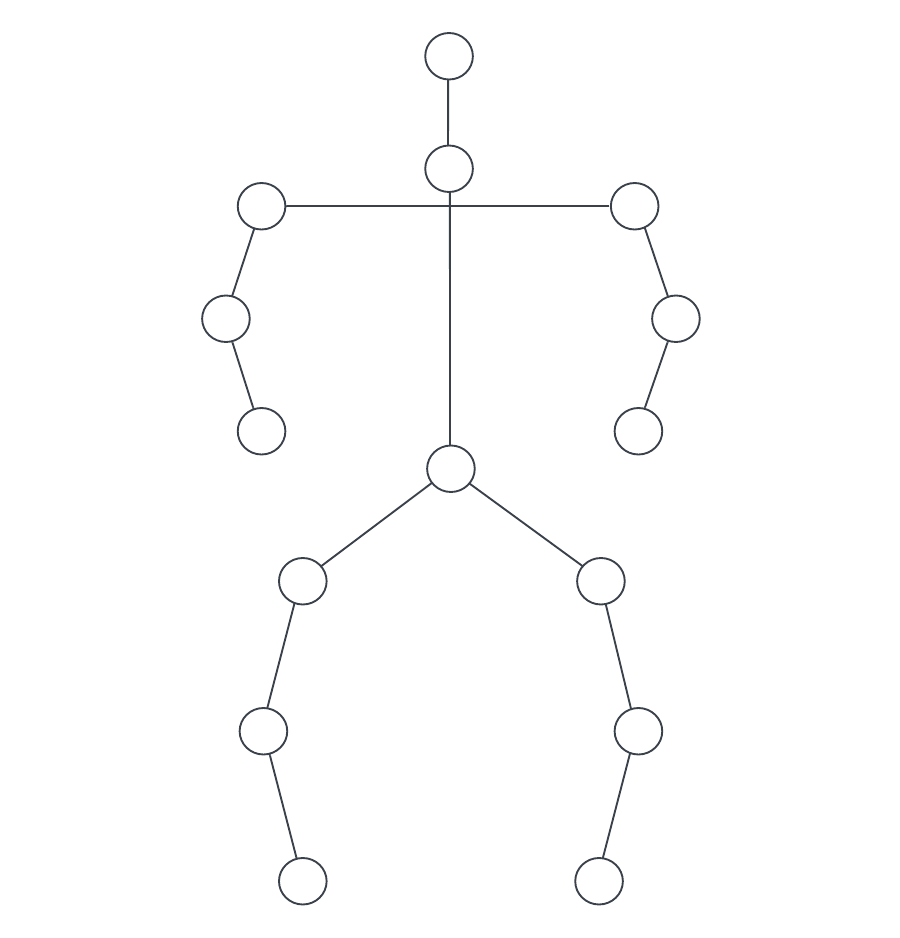
\includegraphics[width=5cm]{pose}
	\centering
	\caption{Example of how joints are connected through bones in pose representations.}
	\label{fig:pose}
\end{figure}

Using the JHMDB dataset, we simply take the existing pose implementation, the representation and indexes being shown in figure \ref{fig:JHMDB}, where there are 15 total joints. Specifically in this thesis, we are concerned with bone-joint-bone connections, effectively representing the angle of the middle joint and how the bones around it move.

\subsection{Joint Angles}

The core of how the new representation will represent actions and movement have to do with the angle between two bones at any one given joint.

\begin{figure}[h]
	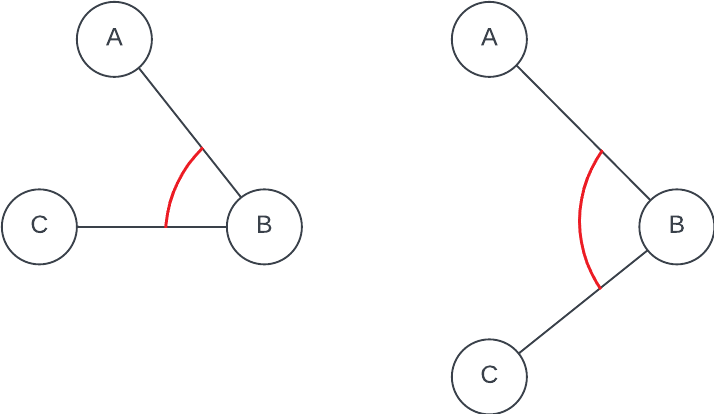
\includegraphics[width=5cm]{JointAngles}
	\centering
	\caption{}
	\label{fig:joint-angles}
\end{figure}

\begin{equation}
	\label{eqn:angle-calculation}
	\centering
	\arctan(a.y/a.x) - \arctan(b.y/b.x)
\end{equation}

\begin{figure}[h]
	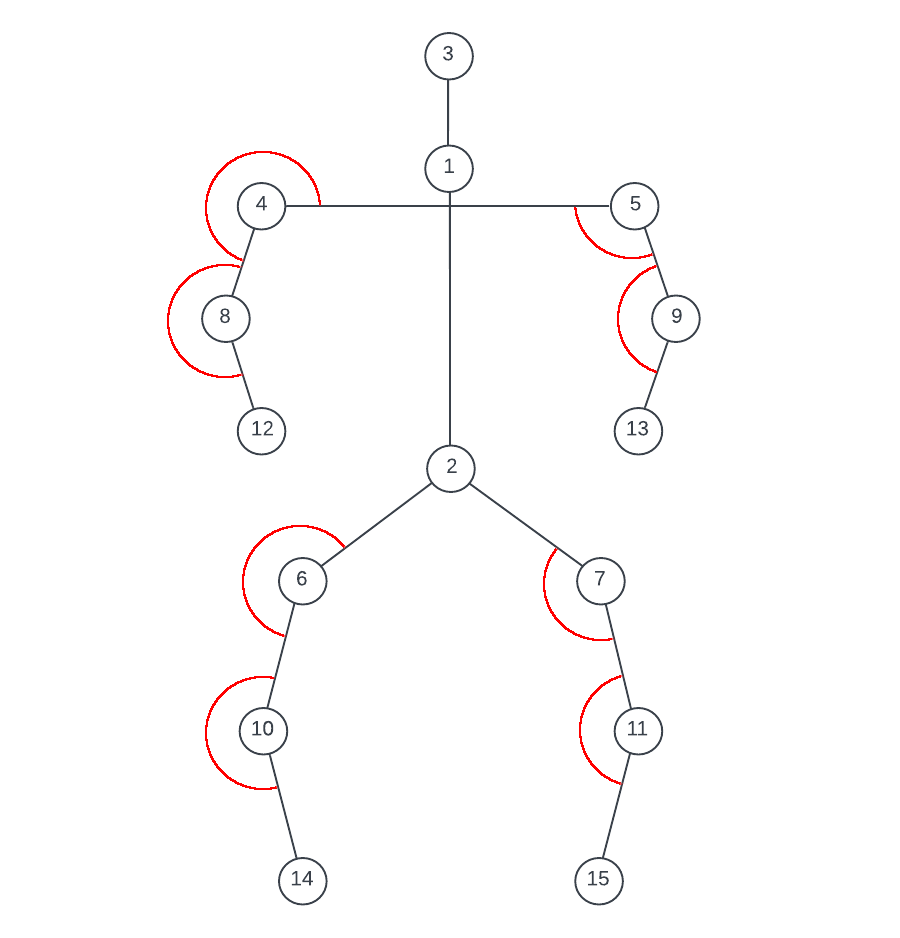
\includegraphics[width=5cm]{PoseJointAngles}
	\centering
	\caption{}
	\label{fig:pose-joint-angles}
\end{figure}

\subsection{Joint Velocities}

\section{Novel Intermediate Representation}

\begin{figure}[h]
	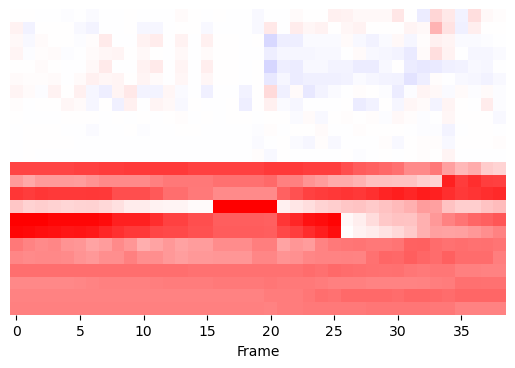
\includegraphics[width=8cm]{IntermediateStacked}
	\centering
	\caption{}
	\label{fig:intermediate-stacked}
\end{figure}

\subsection{Temporal Adjustments}

\begin{figure}
	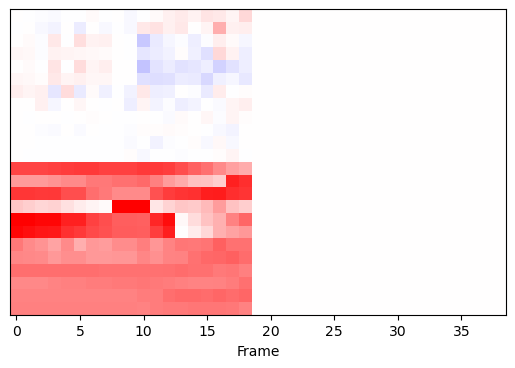
\includegraphics[width=8cm]{IntermediateSkip1}
	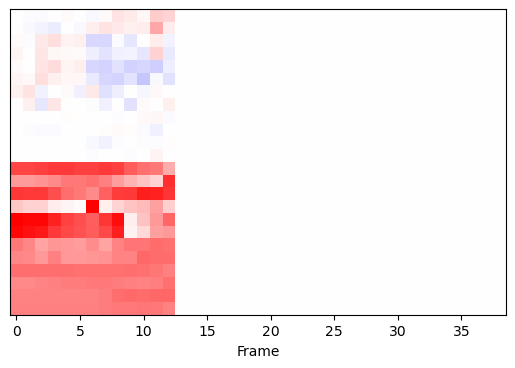
\includegraphics[width=8cm]{IntermediateSkip2}
	\centering
	\caption{}
	\label{fig:intermediate-stacked-skip}
\end{figure}

\subsection{Model Architecture}